\chapter{Competizioni CTF A/D}

Le competizioni CTF di tipo attacco/difesa sono una tipologia di competizioni in cui i partecipanti devono difendere i propri servizi
e attaccare i servizi degli avversari, in un contesto di gara estremamente dinamico e competitivo. 
In queste competizione prendono parte diversi team, i quali vengono associati ogniuno ad una macchina solitamente linux,
con avviati un insieme di servizi che presentano vulnerabilità\footcite{\url{https://faustctf.net/information/attackdefense-for-beginners/}}{faustctf_attackdefense_for_beginners}.
I servizi sono accessibili tramite la rete di gara, e sono replicati su tutte le macchine.

\section{Descrizione dell'infrastruttura}

\subsection{Il Gameserver e i Checker}

Al centro di tutta la competizione c'è il \texttt{gameserver}, entità (che può essere composta da 1 o un insieme di host) che prende in carico
la gestione della competizione eseguento una serie di azioni e fornendo diversi servizi descritti in questo capitolo, essenziali per lo svolgimento della gara stessa.
La competizione è strutturata in \texttt{tick} (o \texttt{round}),
ovvero intervalli di tempo in cui ciclicamente il gameserver assegna punti ai team in base alle azioni compiute dagli stessi
e monitora i servizi tramite i \texttt{checker}.
Questo tempo può variare da competizione a competizione. I \texttt{checker} sono dei bot che si occupano di verificare lo stato della gara eseguendo diverse azioni:
\begin{itemize}
    \setlength{\itemsep}{5pt}
    \setlength{\parskip}{5pt}
    \item Si occupano di verificare se il servizio è funzionante e raggiungibile, andando a connettersi, ed eseguendo azioni
    di normale utilizzo, verificandone anche l'integrita.
    \item Altri si occupano di utilizzare il servizio per memorizzare al suo interno una \texttt{flag}, inserita come informazione sensibile normalmente non accessibile seguendo i normali workflow del servizio.
    \item Altri ancora si occupano di verificare che le flag inserite nei tick precedenti siano ancora raggiungibili tramite un normale accesso autorizzato, e che
    pertanto non siano state modificate o rimosse dal team possessore di quella macchina.
\end{itemize}

In generale, rimuovere vecchie flag, avere il servizio non raggiungibile e non avere la possibilità di inserirne di nuove, sono azioni che vanno ad invalidare la normale
attività del servizio: il gameserver, rilevate queste problematiche, lo andrà a considerare come totalmente o parzialmente inaccessibile o manomesso, dipendentemnte dalle scelte degli organizzatori.\\

Si evidenzia come i checker non sfruttino mai le vulnerabilità dei servizi, ma si limitino al loro corretto utilizzo.

\subsection{I servizi, le flag e i flag store}

Ogni flag viene generata e inserita nel servizio dei vari team ciclicamente ad ogni tick con una sempre flag differente dalle altre, ed ha usualmente una durata massima di valenza (ad esempio 5 tick):
in questo intervallo di tempo è ancora possibile rubare e consegnare la flag al gameserver ottenendo punti.\\

Le flag infatti una volta ottenute vanno consegnate al gameserver, che tramite un calcolo che può variare in diverse competizioni, assegna punti al team che ha consegnato la flag.\\

Nel seguente esempio si mostra il calcolo per l'assegnazione dei punti alla consegna di una flag valida, utilizzato nel progetto CyberChallenge\footcite{\url{https://rules.ad.cyberchallenge.it/}}{cyberchallenge_ad_rules}:

\begin{listing}[H]
    \begin{minted}[
        frame=single,
        framerule=0.8pt,
        fontsize=\footnotesize,
        breaklines
      ]{python}
scale = 15 * sqrt(5) 
norm = ln(ln(5)) / 12 
offense_points[flag] = scale / (1+exp((sqrt(score[attacker][service]) - sqrt(score[victim][service]))*norm))
defense_points[flag] = min(victim_score, offense_points)
\end{minted}
\end{listing}

Il defense point è il punteggio sottratto al team da cui è stata rubata la flag come parte del punteggio di difesa descritto successivamente.\\

\texttt{NOTA:} Si è assunto implicitamente fino ad ora che nè consegnare le flag del proprio team, nè tantomeno
le flag rubate da dei team 'di prova' (spesso chiamati \texttt{NOP team}) possa dare punteggio.
I \texttt{NOP team} sono semplicemente macchine non associate a nessun gruppo reale di persone, che offrono i servizi della gara,
al solo scopo di renderli usufruibili per eseguire penetartion testing (non tutte le competizioni prevedono la presenza dei \texttt{NOP team}).\\
Ciò è possibile poichè il gameserver ha traccia di tutte le flag, di chi le consegna, e delle macchine in cui sono state originariamente inserite dai checker.\\

Una distinzione importante da sottolineare riguarda il significato di \texttt{servizio} di cui si è parlato fino ad ora:
si è implicitamente assunto che per ogni servizio ci sia 1 sola flag per tick e che per ogni servizio ci sia 1 sola vulnerabilità.
Questo spesso non è vero, poichè ogni servizio ha usualmente più vulnerabilità, e non solo, potrebbe avere anche diverse flag per tick a suo interno:
i checker che si occupano di inserire le flag potrebbero inserirne diverse, usando diverse parti o impostazioni del servizio.
In caso di servizi con più flag, diremo che quel servizio conterrà diversi \texttt{flag store}.\\
Ciò detto prima e ciò che verrà detto in seguito è valido per ogni flag store, ma nonostante ciò, continueremo a parlare spesso comunque di servizi per semplicità.\\
\texttt{NOTA:} Comunemente esiste un set di checker differente per ogni flag store.

\subsection{I Flag ID}

Il gameserver potrebbe rilasciare delle informazioni aggiuntive per ogni servizio, come ad esempio un username, che di per se non vanno
ad esporre in maniera diretta ad esempio le credenziali per accedere ad una pagina protetta contenete la flag, ma danno un infomazione utile agli attaccanti al fine di poter
individuare più facilmente la flag all'interno del servizio stesso.
Questa informazione aggiuntiva è chiamata \texttt{Flag ID} e viene rilasciata per ogni team, per ogni flag store, e per ogni flag ancora valida nel momento in cui si visita l'API che
le espone pubblicamente per tutti i partecipanti, resa disponibile dal gameserver. Non è possibile manomettere i flag id, in quanto sono informazioni direttamente rilasciate dagli
organizzatori, che comunque in assenza di vulnerabilità nei servizi, rimangono insufficienti per ottenere flag.

\subsection{Calcolo del punteggio}

Il calcolo del punteggio associato ad ogni team è composto da una serie di punteggi parziali, ogniuno riguardante un servizio.\\
Usualmente ad ogni servizio viene associato un punteggio iniziale di base da cui tutti partono, che viene modificato durante tutta la competizione in base all'
andamento del team relativamente a quel servizio, monitorato a sua volta tramite ulteriori sotto-punteggi che descrivono diversi aspetti del suo andamento.
Le tipologie di punteggi che compongono il punteggio totale del singolo servizio sono descritte in seguito:
\begin{itemize}
    \setlength{\itemsep}{5pt}
    \setlength{\parskip}{5pt}
    \item Il punteggio di \texttt{SLA} (Service Level Agreement) riguarda la disponibilità del servizio, e viene calcolato sulla base di quanto tempo il servizio è stato disponibile o meno.
    Questo è il punteggio che solitamente ha il peso maggiore in assoluto, e spesso viene applicato come percentuale sul totale del punteggio del servizio. Questo accade al fine di
    rendere totalmente insignificante l'idea di spegnere i servizi al fine di evitare di subire attacchi, penalizzando fortemente questa pratica.
    La normale attività del servizio (seppur vulnerabile) pertanto, diventa di vitale importanza nella competizione per tutti i servizi.
    \item Il punteggio di \texttt{attacco} è calcolato sulla base quantitativo di submission di flag valide eseguite dal team. Il punteggio per ogni flag può variare in base alla difficoltà dell'attacco,
    alle condizioni generali di gara e alla velocità con cui si è riusciti ad attaccare quel servizio (come visto nell'esempio precendetemente).
    \item Il punteggio di \texttt{difesa} (solitamente negativo poichè considera quanto "male" ci si sia difesi) è calcolato in base alle consegne
    delle proprie flag eseguite dai team avversari. Accade spesso che questo punteggio vada a controbilanciare il punteggio di attacco sullo stesso servizio, se non a farlo decrescere, andandolo anche a
    portarlo a ribasso del punteggio iniziale assegnato. Esso può essere variabile sulla base degli stessi criteri discussi per il punteggio di attacco. Per questo motivo diventa necessario eseguire
    fix o patch sui propri servizi, impedendo l'arrivo di nuovi attacchi (ma comunque mantenendo il servizio in piena attività),
    e mantenendo l'integrità dei vecchi dati memorizzati (e quindi mantenendo anche le vecchie flag, che se perse andrebbero a deteriorare il punteggio di SLA).
\end{itemize}

\begin{figure}[H]
    \centering
    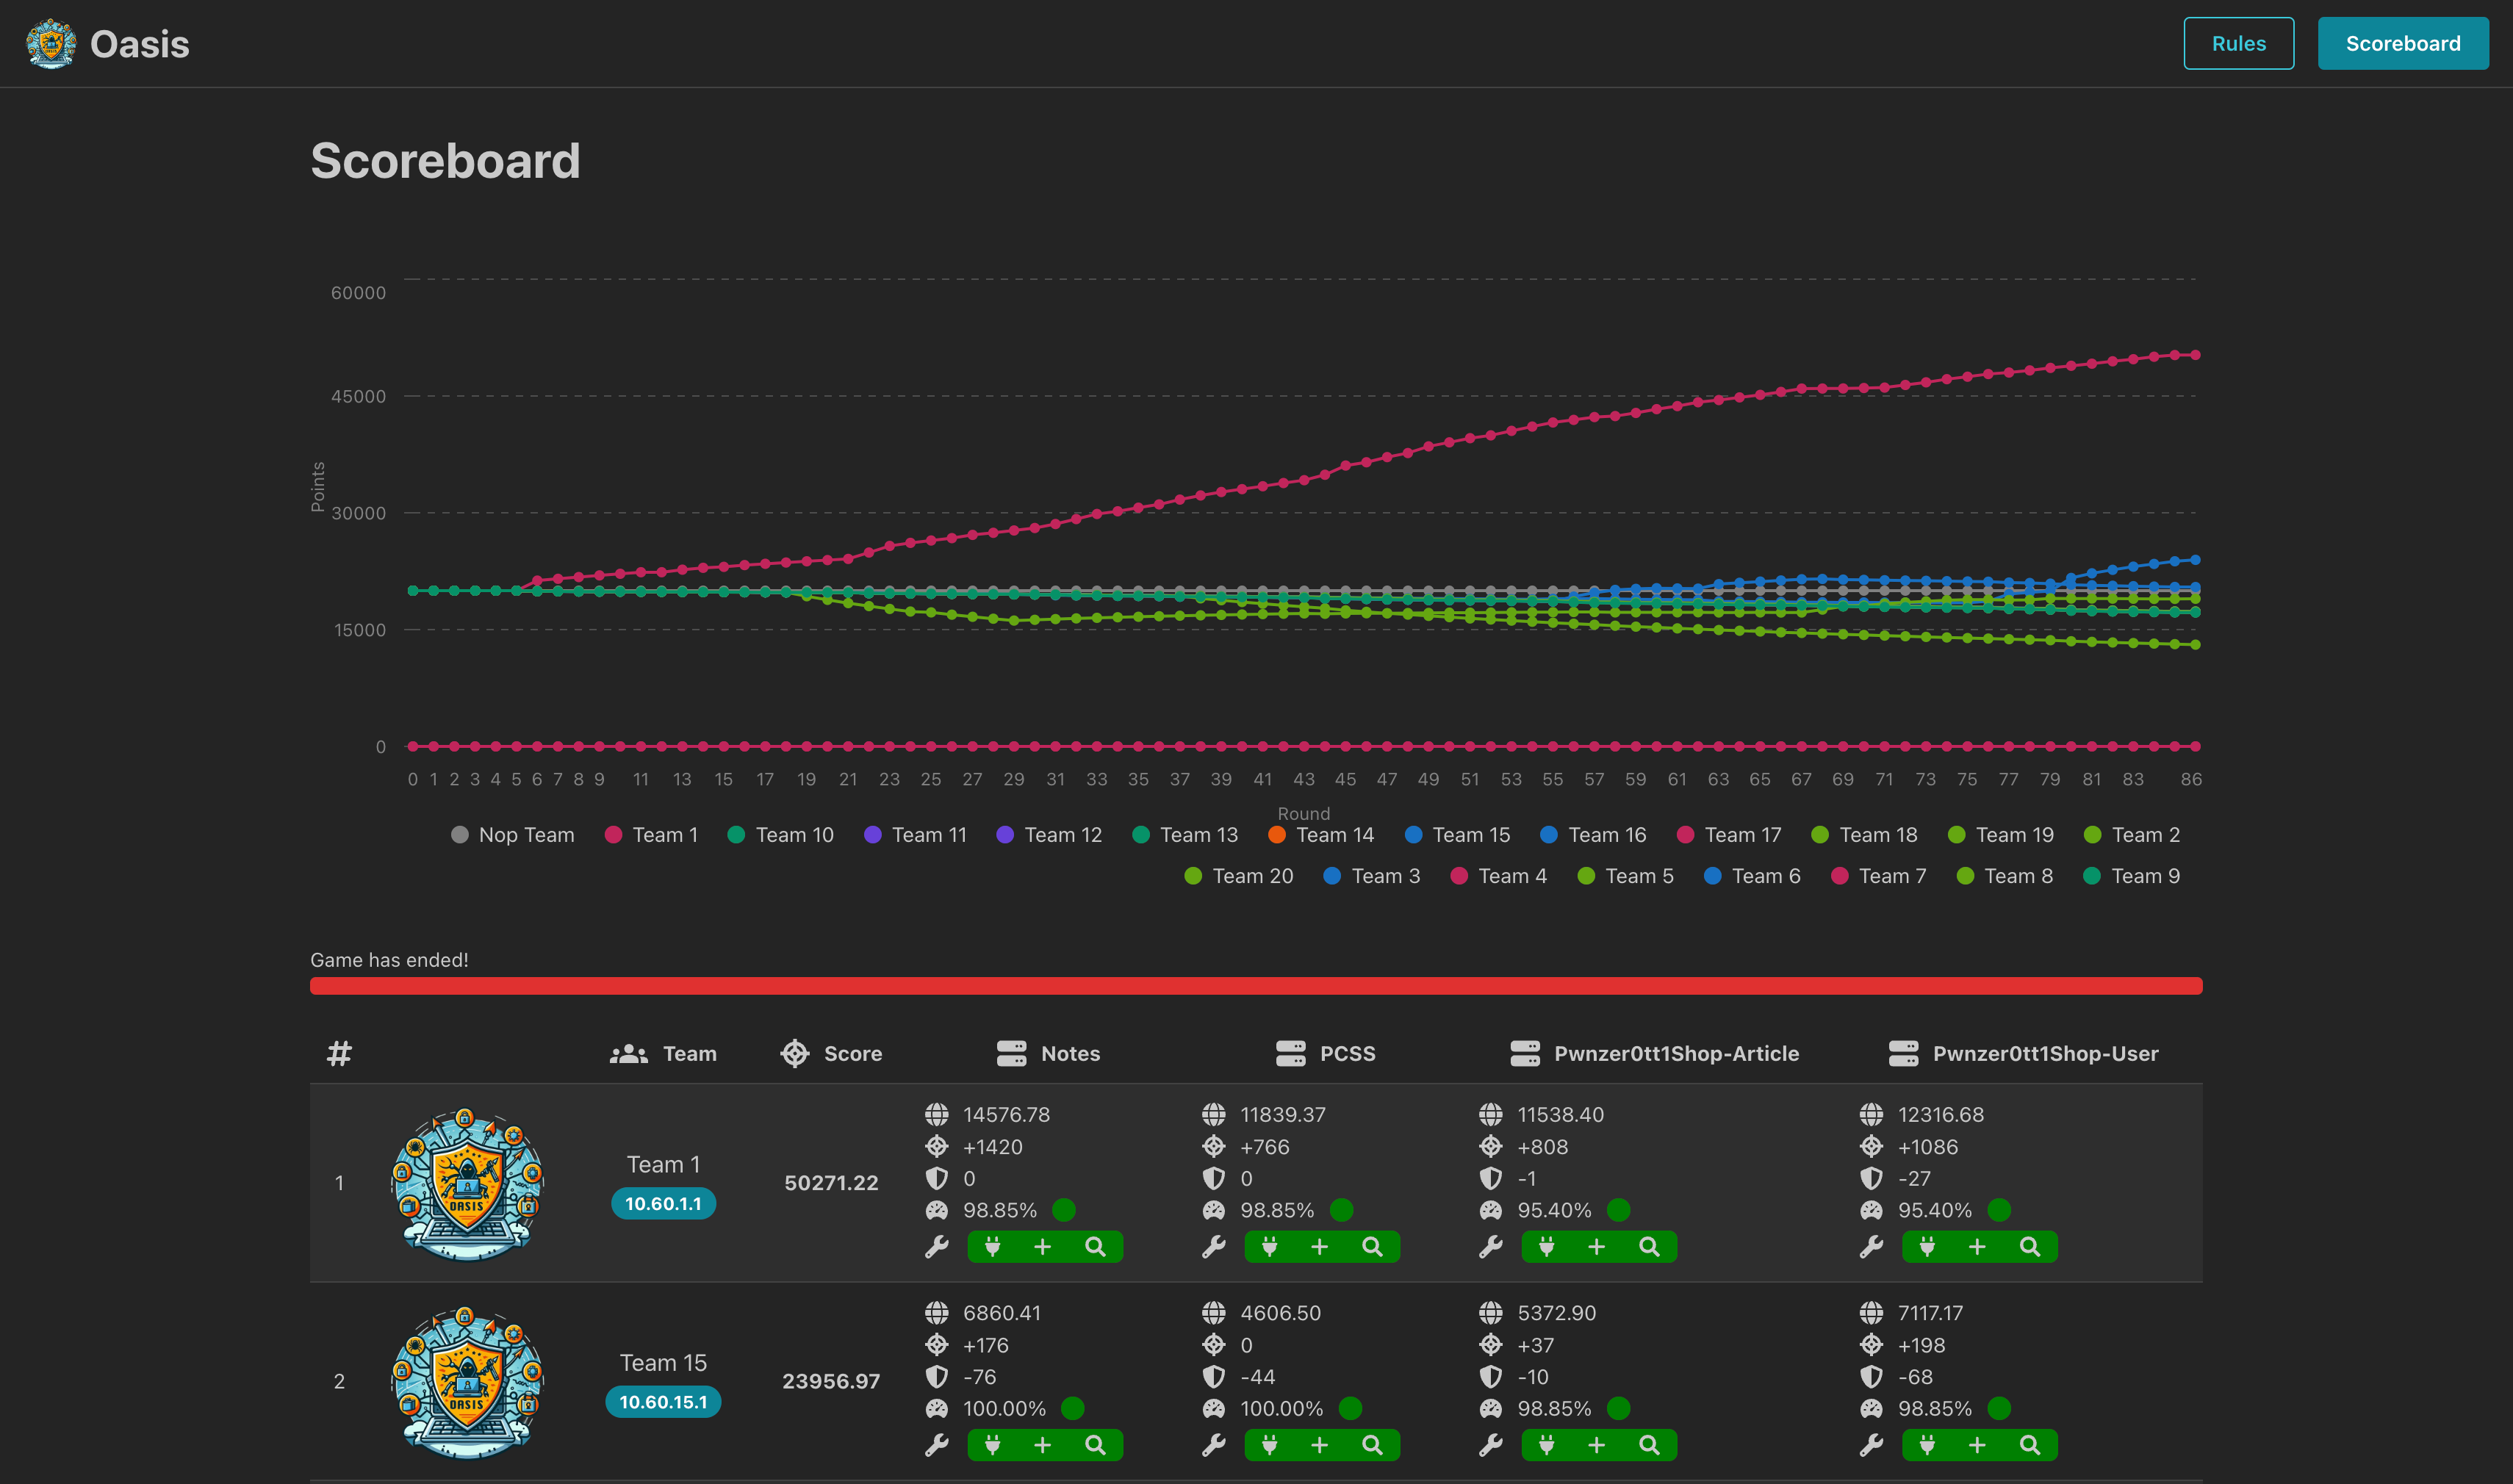
\includegraphics[width=0.85\textwidth]{images/chapter1/oasis_scoreboard.png}
    \caption{Scoreboard di una competizione realizzata con Oasis al DevFest Bari 2024}
    \label{fig:oasis_scoreboard}
\end{figure}

\vspace{\fill}
\newpage

Di seguito si riporta come viene calcolato il punteggio nelle competizioni nazionali attack defence di Cyberchallenge\footcite{\url{https://rules.ad.cyberchallenge.it/}}{cyberchallenge_ad_rules}:

\begin{listing}[H]
    \begin{minted}[
        frame=single,
        framerule=0.8pt,
        fontsize=\footnotesize,
        breaklines
      ]{python}
# --- Total score for each service (or better said, flag store) ---

# Service base points 
score[team][service] = 5000 
            
# Sum offensive points 
for flag in stolen_flags[team][service]:
    score[team][service] += offense_points[flag] 
    
# Substract defensive points 
for flag in lost_flags[team][service]: 
    score[team][service] -= defense_points[flag]

# --- Final team score ---

total_score[team] = 0 
        
for service in services: 
    # Compute SLA of the service
    sla[team][service] = ticks_up[team][service] / ticks[team][service] 
    # Limit scores to 0
    score[team][service] = max(0, score[team][service]) 
    # Add service score
    total_score[team] += score[team][service] * sla[team][service]

\end{minted}
\end{listing}

\newpage

\subsection{Rete di gara}

Per questa analisi si prende in considerazione la rete di gara in utilizzo per le competizioni
nazionali di Cyberchallenge\footcite{\url{https://rules.ad.cyberchallenge.it/}}{cyberchallenge_ad_rules}, sottolineando come 
a grandi linee la configurazione di rete è spesso simile, ma potrebbe variare in base alle competizioni e agli organizzatori.\\

\begin{figure}[H]
    \centering
    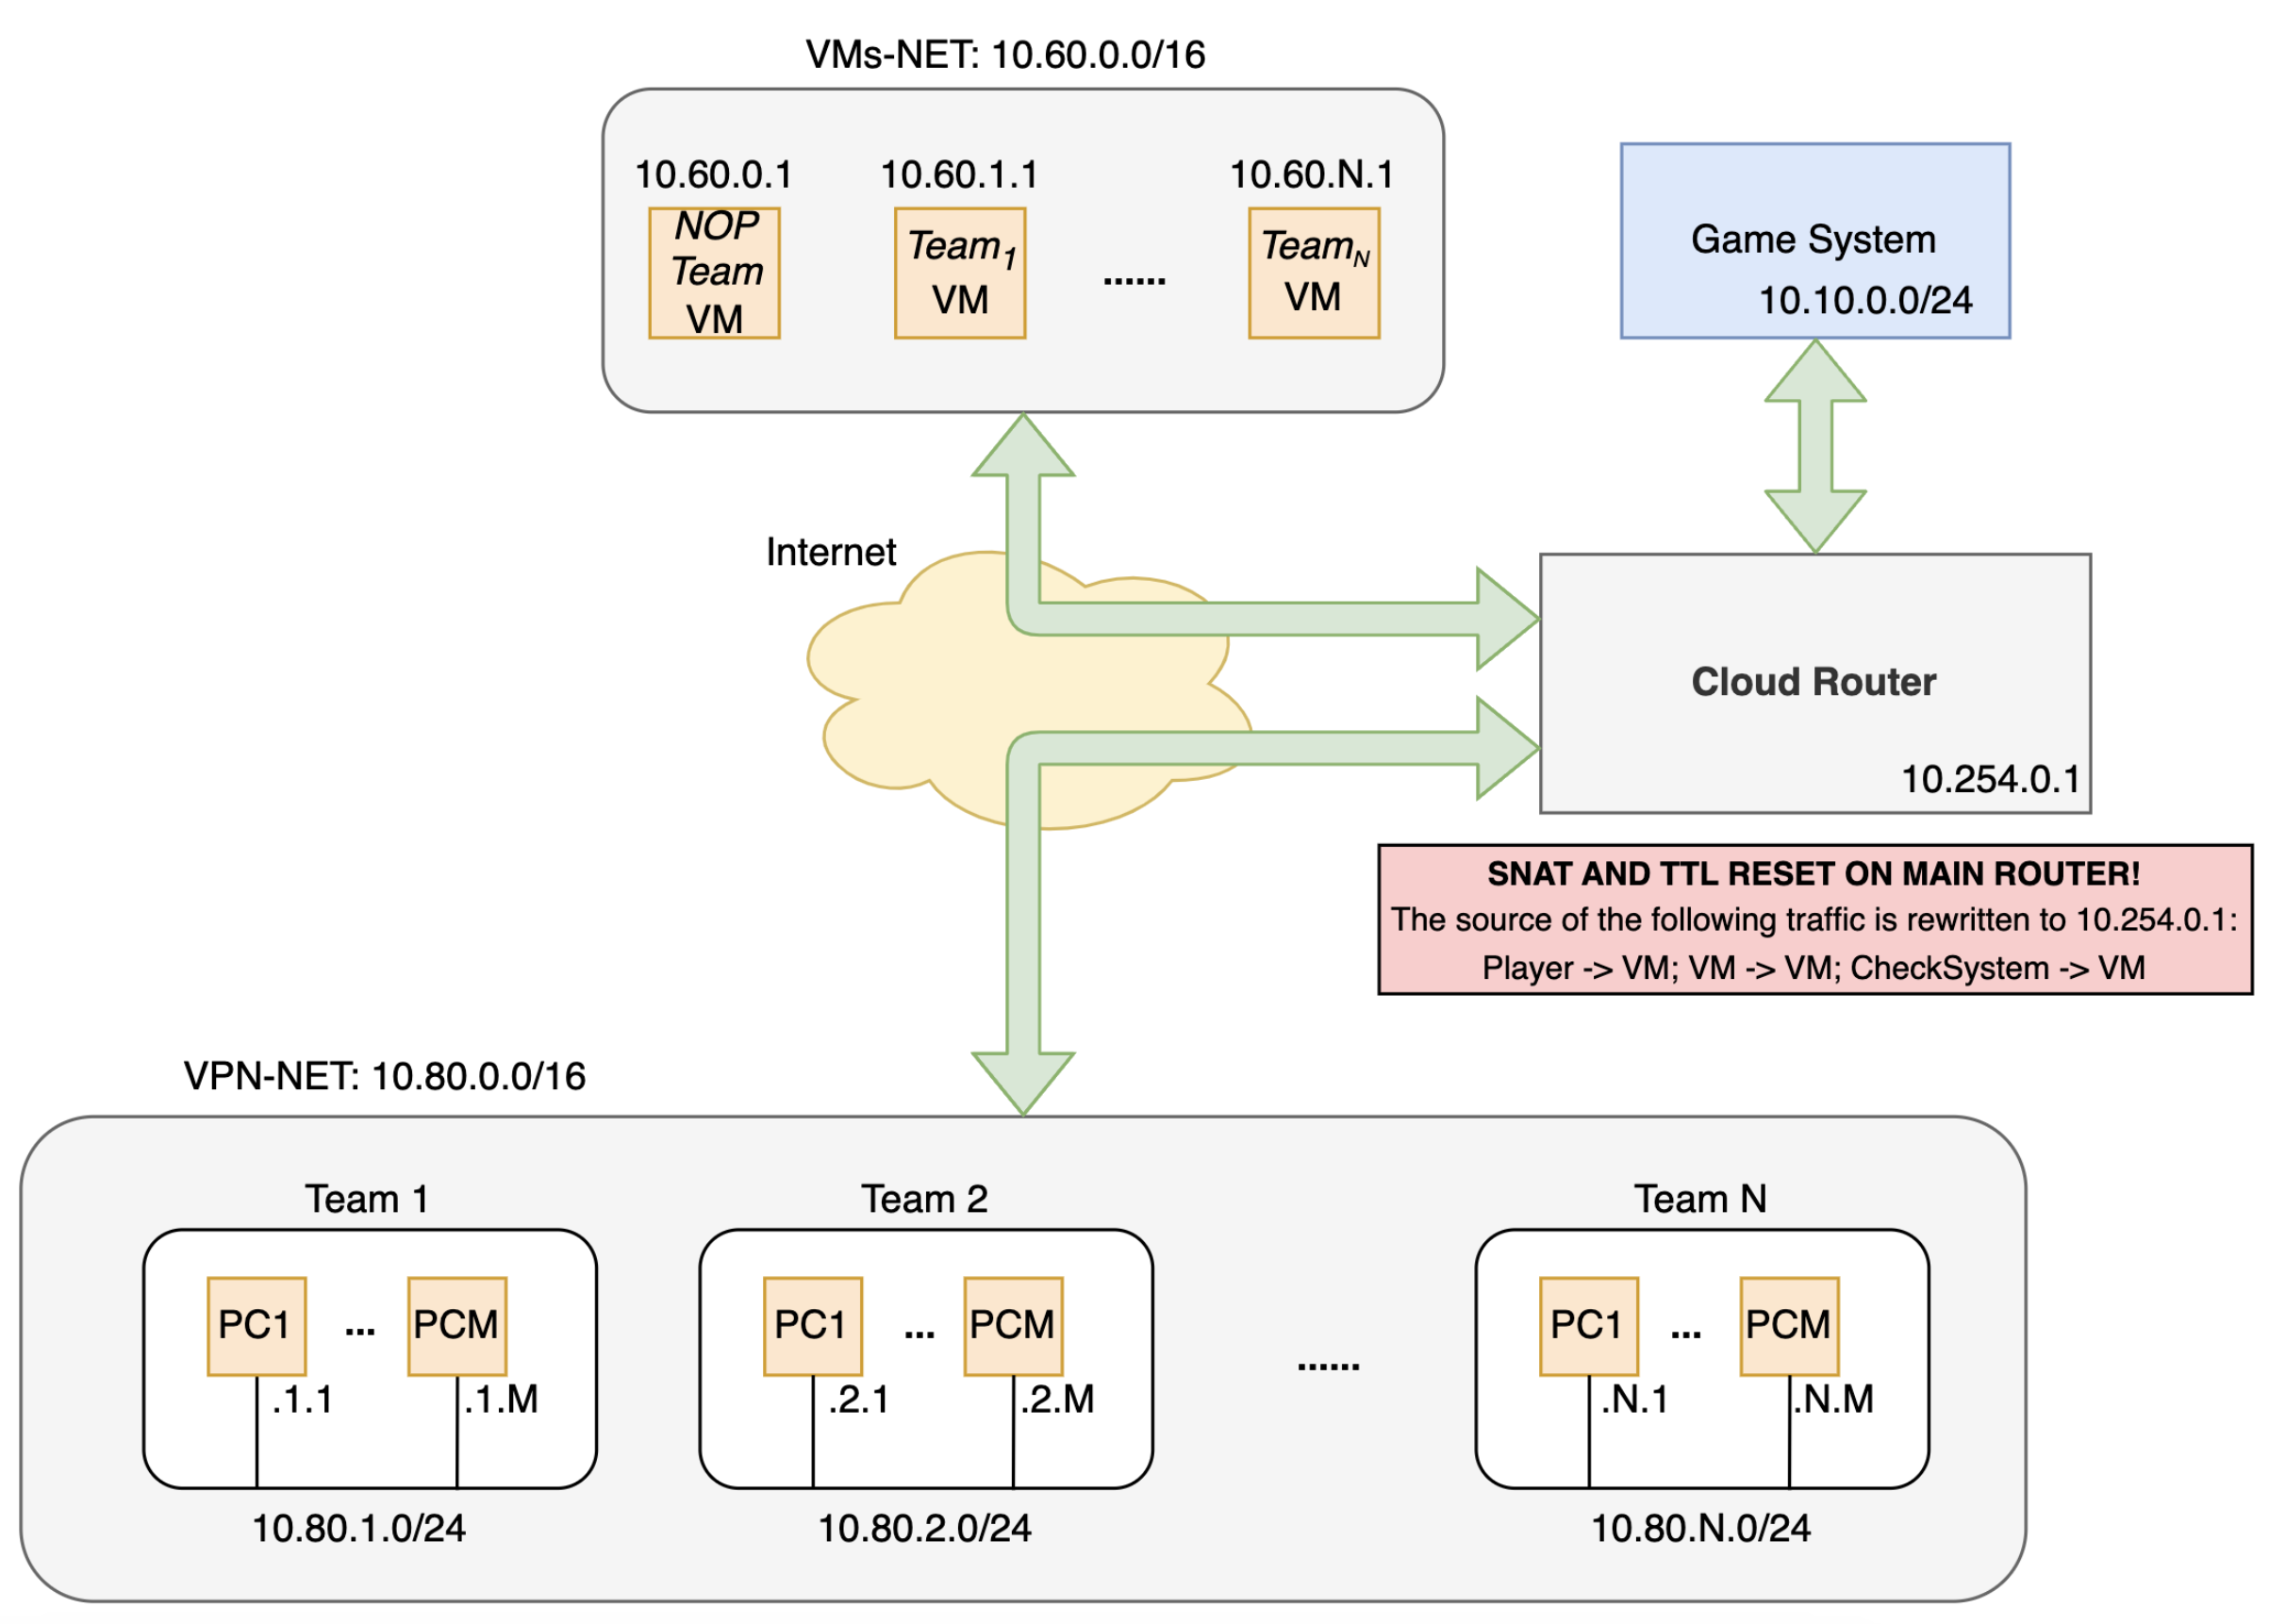
\includegraphics[width=0.8\textwidth]{images/chapter1/ccit_network.png}
    \caption{Modello della rete di gara di Cyberchallenge}
    \label{fig:ccit_network}
\end{figure}

Come si può vedere nella figura \ref{fig:ccit_network} la rete di gara è composta da diversi elementi:
\begin{itemize}
    \setlength{\itemsep}{5pt}
    \setlength{\parskip}{5pt}
    \item La rete dedicata agli organizzatori, dove abbiamo il gameserver (potenzialmente formato da un insieme di host) ed eventuali altri host al servizio degli organizzatori.
    \item La sottorete delle macchine dei team, dove ogni team ha accesso ssh alla propria macchina con i propri servizi vulnerabili.
    \item Una sottorete (spesso realizzata tramite VPN) per ogni team, dove sono connessi gli host dei partecipanti dai quali possono interagire direttamente con la rete di gara.
\end{itemize}

Al centro di tutto ciò troviamo il cloud router, che si occupa di gestire il traffico in base alle regole imposte dagli organizzatori e in base alla fase in cui si trova la competizione,
ma che soprattutto si occupa di \texttt{anonimizzare il traffico} manipolandolo tramite diverse tecniche tra le quali la principale: il \texttt{NAT} (Network Address Translation).
Tramite il \texttt{NAT} infatti si nascondono gli indirizzi IP delle macchine e dei componenti del team, mascherando nelle richieste, l'ip del mittente con quello (o quelli) del router.
Questo è un elemento di fondamentale importanza poichè altrimenti sarebbe davvero molto semplice diversificare le connessioni dei checker e degli attaccanti, e si andrebbe a perdere l'obiettivo che ha
la competizione stessa, ovvero individuare, sfruttare e difendersi dalle vulnerabilità.\\

Inoltre si specifica che le reti dei singoli team sono isolate per tutta la competizione al fine di evitare possibili attacchi agli host dei partecipanti,
che non sono dei target di interesse nella competizione per cui non è possibile e permesso attaccarli.
Un simile comportamento potrebbe portare alla squalifica del team attaccante a seguito di segnalazioni/analisi del traffico da parte degli organizzatori.

\section{Svolgimento della competizione}

Una competizione A/D inizia nel momento in cui viene dato accesso alle macchine e alla rete di gara. Usualmente in questa fase c'è un periodo di tempo
in cui la rete di gara è chiusa: i team hanno accesso unicamente alle loro macchine e nè tramite le macchine stesse nè i componenti del team possono accdere ai servizi degli avversari.\\
È possibile tuttavia già analizzare i servizi, avviare tutti i tool necessari all'avvio degli attacchi, all'analisi della rete, e alla difesa del server (che analizzeremo nel prossimo paragrafo).
Finito questo periodo di tempo, la rete di gara viene aperta, e la competizione inizia ufficialmente.\\
Da ora il gameserver inizia a scandire i tick, i checker iniziano ad utilizzare i servizi e ad inserire le prime flag, pubblicando anche i primi flag id.
I team iniziano a lavorare, tentando di difendersi dai primi attacchi, e a loro volta di attaccare rubando le prime flag agli avversari, tutto ciò manetnendo sempre i loro servizi attivi e funzionanti.
Ad ogni tick, il gameserver assegna i nuovi punteggi, e i team possono osservare tramite questi dati l'evoluzione della gara stessa, comprendendo quali possono essere le azioni da compiere per massimizzare la crescita del loro punteggio.
Inoltre viene segnalato pubblicamente quali dei servizi di quale team non sono funzionanti, e perchè sono considerati down: cioè la motivazione per cui i checker hanno segnalato un mal funzionamento.
La competizione termina ad un determinato orario di fine, dove la rete di gara viene chiusa, e il gameserver interrompe l'azione dei checker non accettando inoltre nuove submission di flag.\\

\texttt{NOTA:} tutto quello descritto in questo paragrafo è possibile simularlo e sperimentarlo tramite un mio progetto chiamato \texttt{Oasis}\footcite{\url{https://github.com/domysh/Oasis}}{oasis_gh},
fork del progetto originale dei TheRomanXpl0it\footcite{\url{https://theromanxpl0.it/about.html}}{theromanxploit} con cui è possibile simulare ma anche 
svolgere una competizione A/D di medio-piccole dimensioni in un ambiente realizzato unicamente tramite l'utilizzo di container, con funzionamento e regolamento simile a quello di CyberChallenge\footcite{\url{https://rules.ad.cyberchallenge.it/}}{cyberchallenge_ad_rules}.

\section{Tool utili}

Data l'elevata complessità nello svolgimento di una competizione A/D, spesso diventa necessario l'utilizzo di tool specializzati che permettano di automatizzare
diverse operazioni necessarie durante la gara. Ogni team può sviluppare e utilizare anche tool che facilitano (o perfino che automizzino) l'attacco e la difesa dei servizi.\\
In generale sono frequenti nel loro utilizzo le seguenti categorie di tool:

\begin{itemize}
    \setlength{\itemsep}{5pt}
    \setlength{\parskip}{5pt}
    \item \texttt{Traffic Analyzer} che permettono di analizzare il traffico sulla macchina, in modo da riconoscere e visionare il traffico dei checker e degli attaccanti (anche se anonimizzato).
    Analizzare il traffico diventa cruciale dal momento in cui un nuovo attacco è attivo sulla rete, poichè permette ai team di analizzarlo, riconoscere la vulnerabilità
    sfruttata, e intraprendere azioni quanto più immediate per la difesa e la replicazione dello stesso attacco. Normalmente per analizzare il traffico è
    possibile usare tool quali \texttt{Wireshark}\footcite{\url{https://www.wireshark.org/}}{wireshark} o \texttt{Suricata}\footcite{\url{https://suricata.io/}}{suricata} (anche se non propriamente un network analyzer).
    Solitamente però non si utilizzano tool simili dato il loro poco pratico utilizzo in ambito CTF A/D dove il traffico da analizzare è elevato e continuo.
    Esistono tool scritti appositamente per queste competizioni che permettono di analizzare il traffico in modo più efficiente e veloce, ma anche di riprodurre velocemente
    le stesse sequenze di attacco, come ad esempio \texttt{Caronte}\footcite{\url{https://github.com/eciavatta/caronte}}{caronte} o
    \texttt{Tulip}\footcite{\url{https://github.com/OpenAttackDefenseTools/tulip}}{tulip} (che utilizza internamente suricata per alcune funzionalità).
    \item \texttt{Attacker \& Submitter} che coordinano gli attacchi, assistono alla scrittura degli exploit, ne monitorano l'esecuzione, schedulandola e parallelizzandola.
    Questi tool sono fondamentali per l'attacco e hanno lo scopo di far focalizzare l'attaccate sulla scrittura del singolo attacco, e non sulla gestione dell'esecuzione di quell'attacco
    su tutte le macchine degli avversari. Inoltre potrebbe esserci in questi tool anche la possibilità di tenere traccia degli attacchi al fine di individuare facilmente problemi nell'esecuzione e 
    monitorare quanti e quali team stanno iniziando a difendere il proprio servizio. Usualmente (ma non sempre) questi tool eseguono anche la parte di submission delle flag al gameserver, che
    (normalmente) avviene in modo centralizzato per tutte le flag ottenute dagli attacchi: questo poichè risulta spesso più semplice coordinarne la consegna, in base alle regole imposte
    dagli organizzatori che ne limitano il numero e la frequenza, al fine di evitare attacchi di tipo \texttt{bruteforce} o \texttt{DoS} all'infrastruttura.
    Tool di questo genere sono ad esempio \texttt{DestructiveFarm}\footcite{\url{https://github.com/DestructiveVoice/DestructiveFarm}}{destructivefarm}, che
    tuttavia ha diversi punti deboli e pecca in diverse funzionalità sull'analisi dell'andamento degli attacchi, motivo per il quale ho sviluppato un nuovo tool chiamato
    \texttt{ExploitFarm}\footcite{\url{https://github.com/Pwnzer0tt1/exploitfarm}}{exploitfarm} che permette di coordinare gli attacchi, di monitorarli, e di schedularli in modo più efficiente e semplice,
    disponendo anche di funzionalità avanzate sulla possibilità di eseguire attacchi distribuiti su più macchine.
    \item \texttt{Proxy e Firewall} che permettono di filtrare il traffico in modo da riconoscere e bloccare gli attacchi. Questi tool possono essere molto utili
    nella difesa, e permettono di bloccare gli attacchi senza di fatto eseguire una modifica sui servizi stessi, spesso causa di malfunzionamenti per errori eseguiti durante questa fase.
    Questo modo di progettere i servizi, tuttavia, è spesso incompleto e superabile, ma se ben progettato e correttamente utilizzato può essere un'ottima soluzione temporanea, se non
    una soluzione completa in alcune casistiche specifiche. Spesso però la soluzione più efficace rimane comunque quella di correggere la vulnerabilità.
    Tool di questo genere sono ad esempio \texttt{CTF Proxy}\footcite{\url{https://github.com/ByteLeMani/ctf_proxy}}{ctf_proxy} o il tool di cui tratta questa tesi \texttt{Firegex}\footcite{\url{https://github.com/Pwnzer0tt1/firegex}}{firegex_gh}.
\end{itemize}

